%%%%%%%%%%%%%%%%%%%%%%%%%%%%%%%%%%%%%%%%%%%%%%%%%%%%%%%%%%%%%%%%%%%%%%%%%%%%%%%%%%%%%
% MARKOV DECISION PROCESSES
%
% Introduction to MDPs, finite MDPs, infinite MDPs
% Semi MDPs
% Partially Observable MDPs
%
%%%%%%%%%%%%%%%%%%%%%%%%%%%%%%%%%%%%%%%%%%%%%%%%%%%%%%%%%%%%%%%%%%%%%%%%%%%%%%%%%%%%%

\section{Markov Decision Processes}
In the face of uncertainty, the agent's \textit{sequential} decision making is formalized in the Markov decision process (MDP). The general MDP framework is shown in Figure \ref{fig:01mdp} and contains two components: the \textbf{agent} and the \textbf{system}. The \textbf{agent} is a continuously learning decision maker and is mathematically represented by the RL algorithm. Objectively, the agent will undergo numerous meaningful interactions with the system to ultimately learn the optimal policy, $\pi^*$ (i.e., the optimal decisions given different situations). Conversely, the \textbf{system} contains all elements the agent cannot arbitrarily control. In process control, the ambient temperature, actuators, and even the wires transporting the control signals are all part of the system because the agent cannot \textit{deterministically} manipulate them. 

\begin{figure}[H]
    \centering
    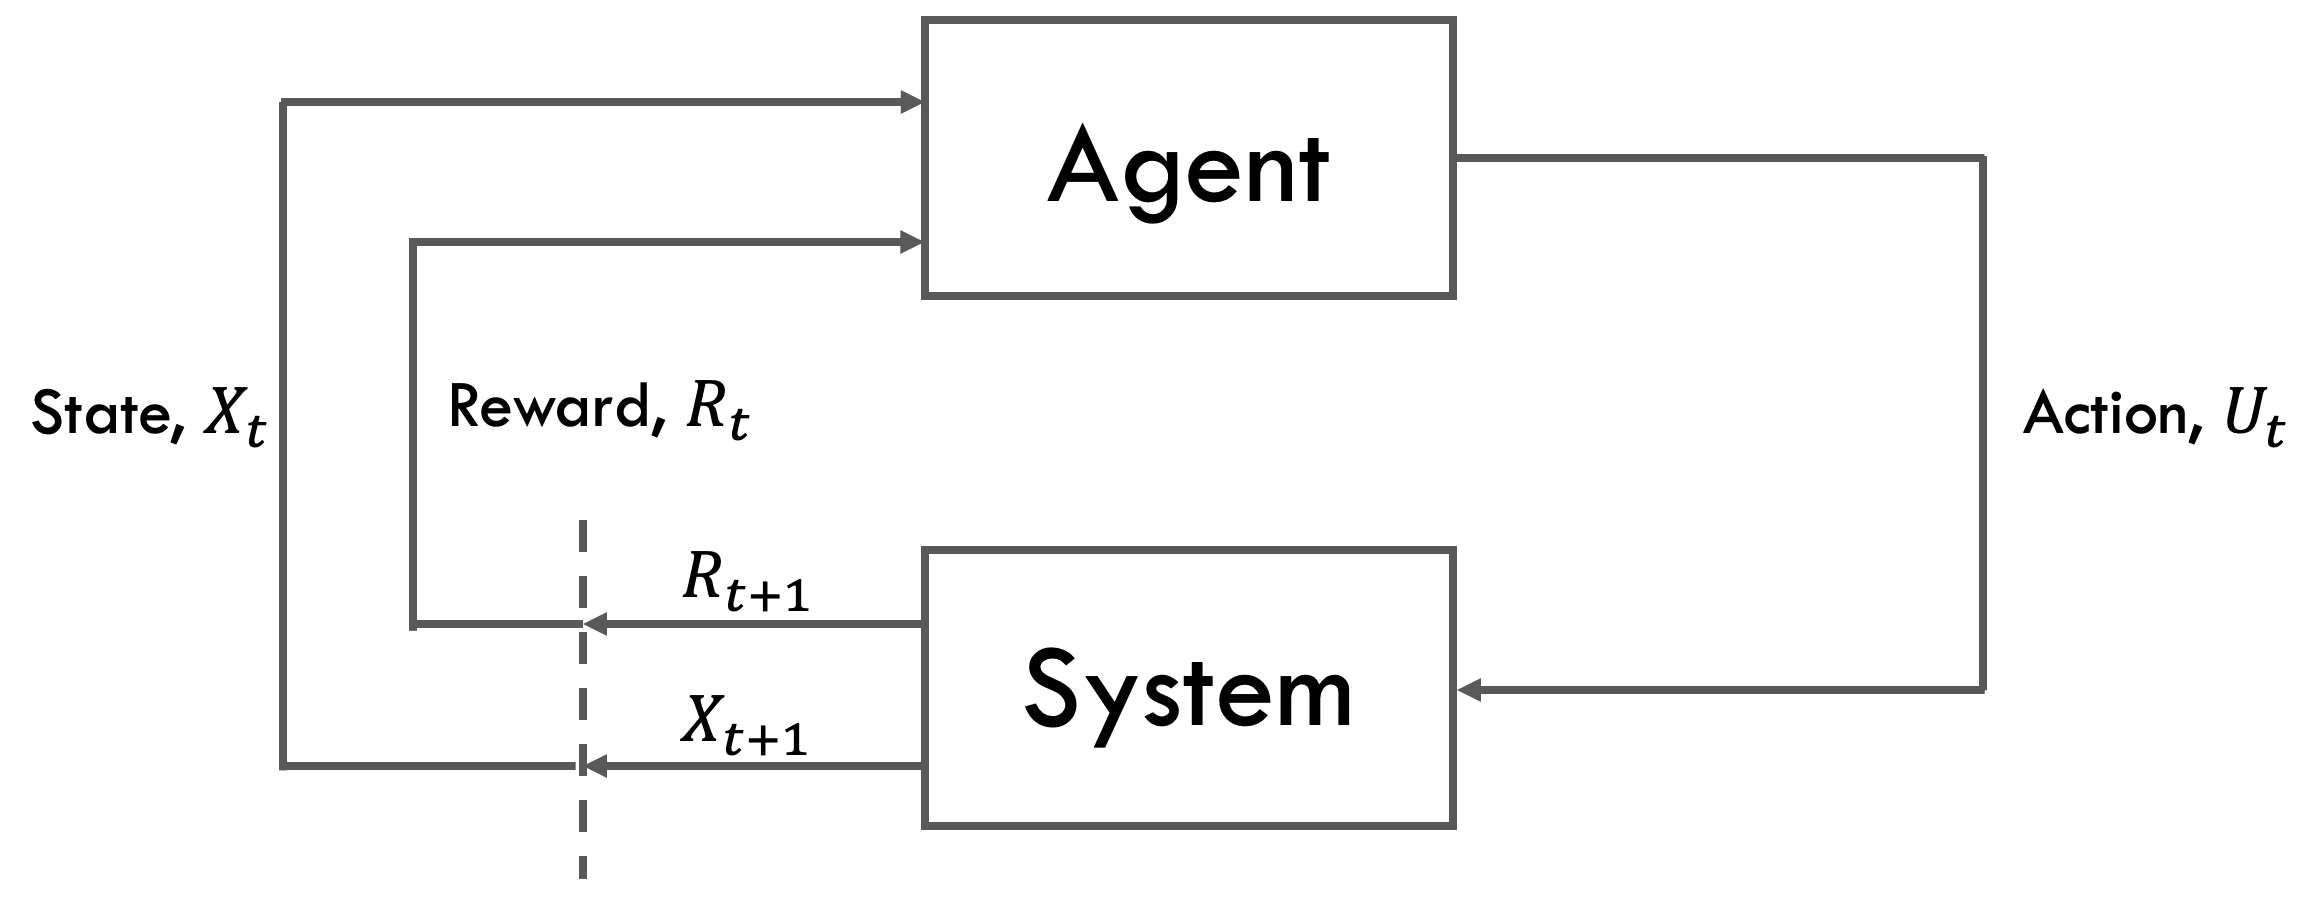
\includegraphics[width=0.56\textwidth]{images/ch1/MDP.jpeg}
    \caption{The general Markov decision process framework. Original image from \cite{sutton}.}
    \label{fig:01mdp}
\end{figure}   

Mathematically, the MDP is a discrete representation of the stochastic optimal problem and a classical formulation of \textit{sequential} decision making where both the immediate and long term consequences are explicitly considered \cite{bellman1, mdp_bellman}. Many definitions of the MDP exist and are equivalent up to small alterations of the process.  One comprehensive definition is that a MDP is a tuple $\mathcal{M}$, is a tuple $(\mathcal{X}, \mathcal{U}$, $P(x', r|x, u), \gamma, R)$ comprised of the following\cite{ng_ref12}:
\begin{itemize}
    \item $x \in \mathcal{X}$: \textbf{State} space of the system at each time step. Common states in industrial processes include temperatures, valve positions, pressures, flow rates, etc.
    \item $u \in \mathcal{U}$: Bounded \textbf{action} space of the agent, ($\mathcal{U}$ $ \geq 2 $). In traditional control, this is the \textbf{bounded input signals} sent to the actuators.
    \item $R \in \mathbb{R}$: Expected \textbf{reward} signal after performing action $u$ in state $x$. Reward functions are designed based on a desired performance metric.  In control theory, the reward function is known as the \textbf{objective function}.  Typically, $|R| \leq \mathcal{R}$ for convergence guarantees.
    \item $p(x', r|x, u)$: Systems \textbf{dynamics function}. Formally, it is the probability of transitioning to $x'$ and receiving $r$,  given states $x \in \mathcal{X}$ and performing action $u \in \mathcal{U}$. Mathematically, it is described by the following:
    \begin{equation}
        p(x', r | x, u) \dot{=} Pr\{X_t = x', R_t = r | X_{t - 1} = x, U_{t-1} = u\}
        \label{eq:transition_prob}
    \end{equation}
    where $p$ describes the system \textbf{dynamics} and $Pr$ denotes the probability operation \cite{sutton}. Additionally, $p$ satisfies the following equality:
    \begin{equation}
        \sum\limits_{x' \in \mathcal{X}} \sum\limits_{r \in \mathcal{R}} p(x', r | x, u) = 1, \forall x \in \mathcal{X}, u \in \mathcal{U}
        \label{eq:prob}
    \end{equation}
    Notice here that $p$ is only a function of the \textit{immediate past}, thus assuming that $x_{t - 1}$ and $u_{t-1}$ captures the complete history. This is known as the Markov property and its underlining assumptions are critical for successful process control applications using RL. Additionally, note that when the state and actions are formulated as augmented past information: $x_{t-1} = [s_{t-1}, s_{t-2}, ... s_{t-N}], u_{t-1} = [a_{t-1}, a_{t-2}, ..., a_{t-N}]$, where $s_{t-N}$ and $a_{t-N}$ denotes the past states and actions, the system is still Markov because decisions can be made exclusively using $x_{t-1}$ and $u_{t-1}$. 
    \item $\gamma$: \textbf{Discount factor} associated with uncertainty of the future, ($0 \leq \gamma \leq 1)$. $\gamma < 1$ is also a requirement for continuous processes to guarantee eventual convergence.
\end{itemize}

There exists three different MDPs: fully observable MDP (FOMDP), partially observable MDP (POMDP), and semi MDP (SMDP). Table \ref{tab:01mdps} shows a general guideline on the different MDPs.

\begin{table}[H]
\caption{A comparison of different Markov decision processes.}
\centering
\begin{tabular}{c|c|c}
\textbf{FO-MDPs}	& \textbf{S-MDPs}	& \textbf{PO-MDPs}\\
\hline
All states observable		  & All states observable			& Some states observable \\
Discrete time		          & Continuous time	             	& Discrete time \\
\end{tabular}
\label{tab:01mdps}
\end{table}

\subsection{Fully observable Markov decision processes}
Fully observable Markov decision processes are the simplest and serves as the foundational framework.  They are mainly applied to discrete systems with fixed sampling times where transition dynamics are unimportant and all states are observable (measurable in control literature). Here, the agent starts in some initial states, $x_0$. At each time $t$, the agent maps $x_t$ to some $u_t$ corresponding to its policy, $\pi_t$.  Given $x_t$ and $u_t$, the system will then transition to some new states $x_{t+1}$ dictated by Equation \ref{eq:transition_prob} while outputting reward signal $R_{t+1}$ based on the reward function. In regulation and set-point tracking problems, this reward function is typically the squared tracking error between $x_t$ and $x_{sp}$.  By repeating this cycle many times, the agent is able to traverse through some sequence, $x_t, u_t, R_{t+1}, x_{t+1}, u_{t+1}, R_{t+2}, x_{t+3}, ...$ and accumulate \cite{sutton}:
\begin{equation}
G_t = R_{t+1} + \gamma R_{t+2} + \gamma^2 R_{t+3} ... = \sum\limits^{\infty}_{k = 0} \gamma^k R_{t+k+1}
\label{eq:return}
\end{equation}
where $G_t$ denotes the cumulative discounted return at time $t$ and $\gamma$ is the discount factor to capture the future uncertainty. MDPs can represent both finite or infinite systems; the former describes episodic tasks with explicit terminal states while the latter describes tasks that continue forever.  Intuitively, most two-player board games such as Checkers, Chess, or Go are finite MDPs where the game is terminated after one player is defeated.  Contrarily, an infinite MDP system could be the control system in an industrial process. For infinite MDP systems, $\gamma < 1$ is a necessary condition to keep $G_t$ bounded. Ultimately, the agent is tasked with finding the optimal policy, $\pi^*$, that maximize $G_t$, and subsequently the value function, over $N$ steps. The value function for each state is given as \cite{sutton}:
\begin{equation}
    v_\pi (x) \dot{=} \mathbb{E}_\pi [G_t | X_t = x] = \mathbb{E}_\pi \left[\sum\limits^\infty_{k=0} \gamma^k R_{t+k+1} | X_t = x \right] = \mathbb{E}_\pi [R_{t+1} + \gamma G_{t+1} | X_t = x]
    \label{eq:value_func}
\end{equation}
$$\forall x \in \mathcal{X}$$
where $v_\pi (s)$ is the value function of state $x$ under policy $\pi$. Additionally, $v_{\pi}$ is guaranteed to exist and be unique for continuous systems where $\gamma < 1$ or in systems with guaranteed termination.  Compared to Equation \ref{eq:karmed}, Equation \ref{eq:value_func} takes the expectation of $G_t$ (defined in Equation \ref{eq:return}) rather than $R_t$; therefore, optimizing the long term trajectory compared to only immediate rewards. The action-value version of Equation \ref{eq:value_func} is given as:
\begin{equation}
    q_\pi (x, u) \dot{=} \mathbb{E}_\pi [G_t | X_t = x, U_t = u] = \mathbb{E}_\pi \left[\sum\limits^\infty_{k=0} \gamma^k R_{t+k+1} | X_t = x, U_t = u \right], \forall x, u \in \mathcal{X, U}
    \label{eq:a_value_func}
\end{equation}
FOMDPs can find the optimal policy for systems where all states are observable.  Unfortunately, there are often times where states are unobservable (unmeasurable in control) due to hardware limitations or other factors. During such situations, the system no longer exhibits the Markov property ultimately resulting in sub-optimal decision making.


\subsection{Semi Markov Decision Processes}

\subsection{Partially Observable Markov Decision Processes}
